\documentclass[12pt,a4paper]{article}
\renewcommand{\thesection}{\Roman{section}}
\renewcommand{\thesubsection}{\thesection.\Roman{subsection}}
\usepackage{xeCJK}
\usepackage{amssymb}
\usepackage{amsmath}
\usepackage{geometry}
\usepackage{subfig}
\usepackage{fancyhdr}
\usepackage[export]{adjustbox}
\usepackage{graphicx}
\graphicspath{{images/}}
\geometry{left=2.5cm,right=1.5cm,top=2cm,bottom=2cm}

\title{Deep Learning and Practice \\Lab1 \\ Report}
\date{March 28, 2019}
\author{呂紹篁, 0751904}
\setCJKmainfont{AR PL UKai CN}
\begin{document}
\thispagestyle{plain}
\cfoot{}
\maketitle


\section{Introduction} \label{sec:intro}
In this lab, we are assigned to implement a neural network with two hidden layers, while some firmwares such as Tensorflow, Pytorch, are not allowed to used. We are given two datasets to do the classification work, both with 2-channel input and 2 classes, either 0 or 1. One dataset is linear separable, i.e., we can find a line in ${\mathbb{R}}^2$ that separate two groups perfectly. The other dataset, which we called it \textbf{XOR Dataset}, doesnot have the feature, and hence we cannot find such line to separate the data. \\
Nevertheless, we still can use our model to predict the class of the given data with the power of neural network. First, we have to design our model, initialize the weights of it arbitrarily, and define the loss function to measure how good of our model is. Second, we throw the data into the model, get the prediction result and the loss. With these information, we can compute the gradient of the loss surface with respect to all weights in the model and update the weight by the method called \textbf{gradient descent}. The process will continue until the result is acceptable. \\
The reminder of this report is organized as below. In Section~\ref{sec:exp} we detaily describe our methods, Section~\ref{sec:res} illustrate the result of testing, and some discussions are proposed in Section~\ref{sec:discuss}.
\section{Experiment Setups} \label{sec:exp}
\subsection{Sigmoid functions}
To increase the nonlinearity of the model, several activation functions will be inserted to the model.  There are several activation functions available, for example, ReLU (rectified linear unit), TanH and Sigmoid. In this lab, we use Sigmoid as our activation function, which is defined in Equation~\ref{eq: sigmoid}. The derivative of Sigmoid can be expressed as Equation~\ref{eq: derivative_sigmoid}.

\begin{equation} \label{eq: sigmoid}
  \sigma(x) = \frac{1}{1+exp(-x)}
\end{equation}

\begin{equation} \label{eq: derivative_sigmoid}
  \sigma'(x) = \sigma(x)*(1-\sigma(x))
\end{equation}
\subsection{Neural Network}
The archietecture of the model is illustrated as Fig.~\ref{fig:nn_arch}. There are two hidden layers with 2-channel input 2-channel output, and one output layer with 2-channel input 1-channel output. To simplify the work, all layers are without bias. The activation functions are inserted behind each layer. We use \textbf{cross entropy} as loss function which is described in Equation~\ref{eq: cross_entropy}. The intuitive expression of cross entropy is to measure the distance between two distinguish distributions and is suitable to use in classification model.

\begin{equation} \label{eq: cross_entropy}
  Loss = -(y*\log(y\_pred) + (1-y)*\log(1-y\_pred))
\end{equation}
\subsection{Backpropagation}
To get better prediction result, we use \textbf{gradient descent} to find the best weight of our model. Imaging that we are at a high mountain and want to reach a location with lowest altitude, we will look around, find the best direction and follow it until we reach the flatten plane. The best direction and the mountain, in Mathematic terminology, is called gradient and loss hypersurface respectively. To compute the gradients effectively, we use the algorithm called \textbf{backpropagation}. The key idea is the \textbf{chain rule} in \textit{Calculus}. All 10 gradients are expressed as followings after some derivation.

\begin{eqnarray}
  \left\{
  \begin{aligned}
    \frac{\partial L}{\partial w_1} = \frac{\partial L}{\partial y\_pred} * \frac{\partial y\_pred}{\partial z_3} * \frac{\partial z_3}{\partial w_1} \\
    \frac{\partial L}{\partial w_2} = \frac{\partial L}{\partial y\_pred} * \frac{\partial y\_pred}{\partial z_3} * \frac{\partial z_3}{\partial w_2}
  \end{aligned}
  \right.
  \label{eq: L_to_W3}
\end{eqnarray}

\begin{eqnarray}
  \left\{
  \begin{aligned}
    \frac{\partial L}{\partial w_\text{31}} = \frac{\partial L}{\partial y\_pred} * \frac{\partial y\_pred}{\partial z_3} * \frac{\partial z_3}{\partial a_\text{21}} * \frac{\partial a_\text{21}}{\partial z_\text{21}} * \frac{\partial z_\text{21}}{\partial w_\text{31}} \\
    \frac{\partial L}{\partial w_\text{32}} = \frac{\partial L}{\partial y\_pred} * \frac{\partial y\_pred}{\partial z_3} * \frac{\partial z_3}{\partial a_\text{22}} * \frac{\partial a_\text{22}}{\partial z_\text{22}} * \frac{\partial z_\text{22}}{\partial w_\text{32}} \\
    \frac{\partial L}{\partial w_\text{41}} = \frac{\partial L}{\partial y\_pred} * \frac{\partial y\_pred}{\partial z_3} * \frac{\partial z_3}{\partial a_\text{21}} * \frac{\partial a_\text{21}}{\partial z_\text{21}} * \frac{\partial z_\text{21}}{\partial w_\text{41}} \\
    \frac{\partial L}{\partial w_\text{42}} = \frac{\partial L}{\partial y\_pred} * \frac{\partial y\_pred}{\partial z_3} * \frac{\partial z_3}{\partial a_\text{22}} * \frac{\partial a_\text{22}}{\partial z_\text{22}} * \frac{\partial z_\text{22}}{\partial w_\text{42}} \\
  \end{aligned}
  \right.
  \label{eq: L_to_W2}
\end{eqnarray}

\begin{eqnarray}
  \left\{
  \begin{aligned}
    % 11
    \frac{\partial L}{\partial w_\text{11}} = \frac{\partial L}{\partial y\_pred} * \frac{\partial y\_pred}{\partial z_3} * \frac{\partial z_3}{\partial a_\text{21}} * \frac{\partial a_\text{21}}{\partial z_\text{21}} * \frac{\partial z_\text{21}}{\partial a_\text{11}} * \frac{\partial a_\text{11}}{\partial z_\text{11}} * \frac{\partial z_\text{11}}{\partial w_\text{11}} \\ + 
      \frac{\partial L}{\partial y\_pred} * \frac{\partial y\_pred}{\partial z_3} * \frac{\partial z_3}{\partial a_\text{22}} * \frac{\partial a_\text{22}}{\partial z_\text{22}} * \frac{\partial z_\text{22}}{\partial a_\text{11}} * \frac{\partial a_\text{11}}{\partial z_\text{11}} * \frac{\partial z_\text{11}}{\partial w_\text{11}} \\
    % 12
    \frac{\partial L}{\partial w_\text{12}} = \frac{\partial L}{\partial y\_pred} * \frac{\partial y\_pred}{\partial z_3} * \frac{\partial z_3}{\partial a_\text{21}} * \frac{\partial a_\text{21}}{\partial z_\text{21}} * \frac{\partial z_\text{21}}{\partial a_\text{12}} * \frac{\partial a_\text{12}}{\partial z_\text{12}} * \frac{\partial z_\text{12}}{\partial w_\text{12}} \\ + 
      \frac{\partial L}{\partial y\_pred} * \frac{\partial y\_pred}{\partial z_3} * \frac{\partial z_3}{\partial a_\text{22}} * \frac{\partial a_\text{22}}{\partial z_\text{22}} * \frac{\partial z_\text{22}}{\partial a_\text{12}} * \frac{\partial a_\text{12}}{\partial z_\text{12}} * \frac{\partial z_\text{12}}{\partial w_\text{12}} \\
    % 21
    \frac{\partial L}{\partial w_\text{21}} = \frac{\partial L}{\partial y\_pred} * \frac{\partial y\_pred}{\partial z_3} * \frac{\partial z_3}{\partial a_\text{21}} * \frac{\partial a_\text{21}}{\partial z_\text{21}} * \frac{\partial z_\text{21}}{\partial a_\text{11}} * \frac{\partial a_\text{11}}{\partial z_\text{11}} * \frac{\partial z_\text{11}}{\partial w_\text{21}} \\ + 
      \frac{\partial L}{\partial y\_pred} * \frac{\partial y\_pred}{\partial z_3} * \frac{\partial z_3}{\partial a_\text{22}} * \frac{\partial a_\text{22}}{\partial z_\text{22}} * \frac{\partial z_\text{22}}{\partial a_\text{11}} * \frac{\partial a_\text{11}}{\partial z_\text{11}} * \frac{\partial z_\text{11}}{\partial w_\text{21}} \\
    % 22
    \frac{\partial L}{\partial w_\text{22}} = \frac{\partial L}{\partial y\_pred} * \frac{\partial y\_pred}{\partial z_3} * \frac{\partial z_3}{\partial a_\text{21}} * \frac{\partial a_\text{21}}{\partial z_\text{21}} * \frac{\partial z_\text{21}}{\partial a_\text{11}} * \frac{\partial a_\text{11}}{\partial z_\text{11}} * \frac{\partial z_\text{11}}{\partial w_\text{22}} \\ + 
      \frac{\partial L}{\partial y\_pred} * \frac{\partial y\_pred}{\partial z_3} * \frac{\partial z_3}{\partial a_\text{22}} * \frac{\partial a_\text{22}}{\partial z_\text{22}} * \frac{\partial z_\text{22}}{\partial a_\text{11}} * \frac{\partial a_\text{11}}{\partial z_\text{11}} * \frac{\partial z_\text{11}}{\partial w_\text{22}} \\
  \end{aligned}
  \right.
  \label{eq: L_to_W1}
\end{eqnarray}

Through the result seems complicated, there are several common terms which can simplify the expressions. \\
After we get the gradients, we can update the weights with ${w^*_\text{ij} = w_\text{ij} - \eta \frac{\partial L}{\partial w_\text{ij}}}$ where ${\eta}$ is learning rate. \\
There are several deformation of gradient desent. In this lab, we use \textbf{mini-batch} with batch size equals to 1, i.e., update weights after each data. The learning rate of both models are constant with value 0.01 after fine tune, and since the Separable Dataset is easier to train, we use only 10000 epochs while 200000 epochs for XOR Dataset. We didnot shuffle the order of training data.

\begin{figure}[t!]
  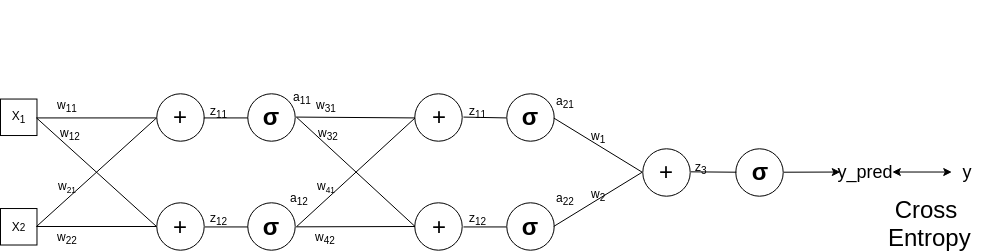
\includegraphics[scale=0.35]{DLP_report1_nn.png}
  \centering
  \caption{Design of Neural Network Architecture}
  \label{fig:nn_arch}
\end{figure}

\section{Results of testing} \label{sec:res}
\subsection{Screenshot and Comparison Figure}
\begin{figure}[t]
  \centering
  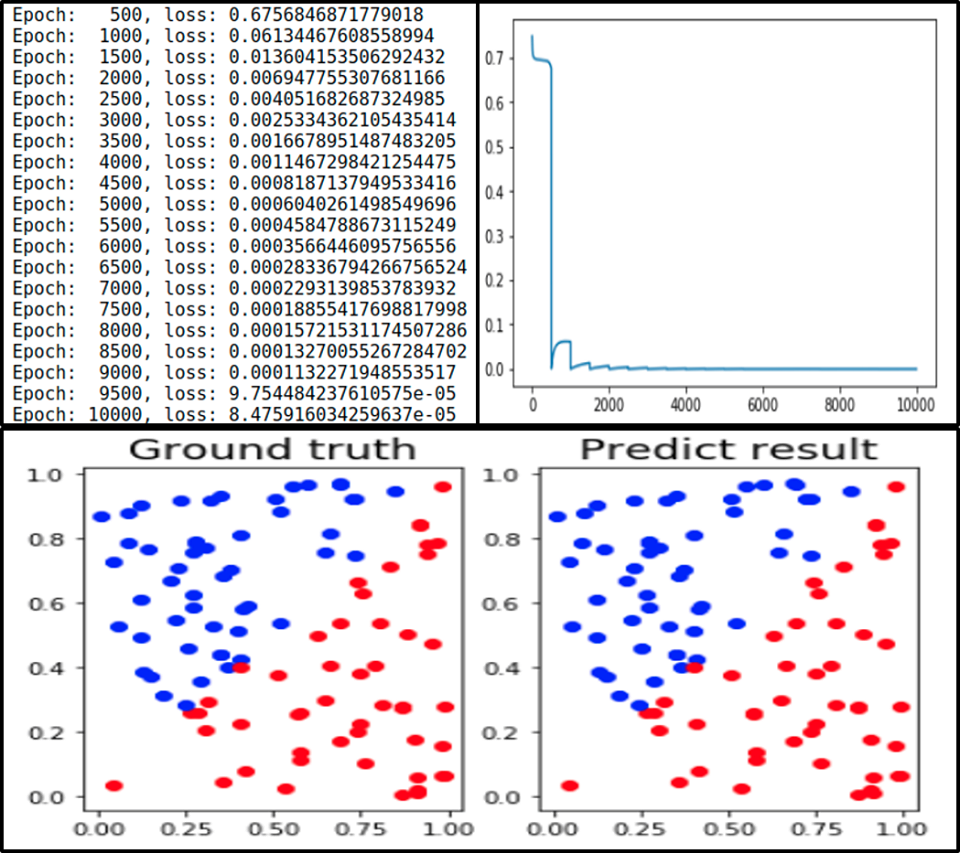
\includegraphics[scale=0.26]{separable_all.png}
  \caption{Separable Dataset Training and Testing Result}
  \label{fig:ls_res}
\end{figure}
\begin{figure}[t]
  \centering
  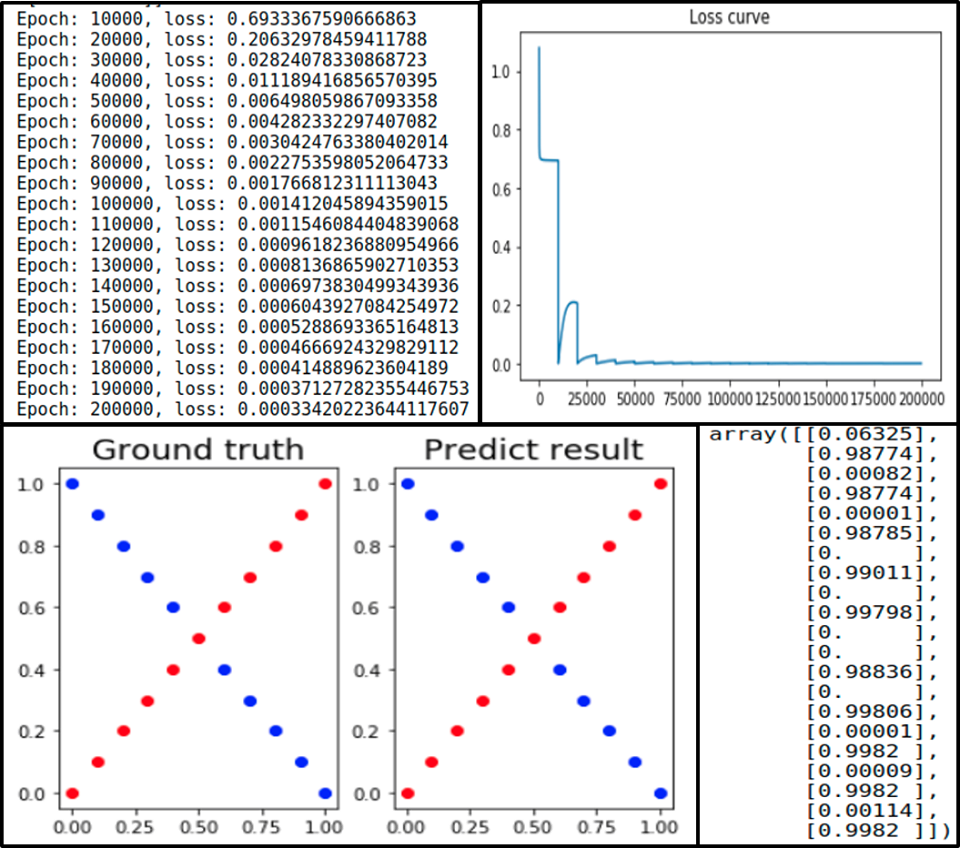
\includegraphics[scale=0.26]{xor_all.png}
  \caption{XOR Dateset Training and Testing Result}
  \label{fig:xor_res}
\end{figure}
The training and Testing results of two dataset are summarized in Fig~\ref{fig:ls_res} and Fig~\ref{fig:xor_res}. Output of training, loss curve and comparison of ground truth are provided. 
\subsection{Loss Curve}
From the loss curves we can notice that the loss declined rapidly after few epochs. The loss keep decreasing and start to oscillate when close to 0. However, from the output of training, the tendency of the loss indeed decreasing which tell us that our model is learning.
\subsection{Effect of Learning Rate}
To understand the effect of learning rate, we try 5 different values with same weight initialization and provide the loss curves and prediction results against XOR Dataset. The results are shown in Fig~\ref{fig:lr_com}. From the result, we can find that [0.1, 0.01] may be the best range of learning rate. Large or small learning rate may cause the huge amplitude of oscillation.
\subsection{Effect of Weight Initialization}
With the same network archietecture and the same hyperparameters, different weight initialization may also get the different results. We use four criterions to test the affect of weight initialization and the loss curve results are provided in Fig~\ref{fig:init}. In first row, we can notice that two curves are similar besides begining epochs. In second row, as expected, with huge initialization, the model is hard to converge with same epochs. If the initialization is close to the good model, the loss is very tiny and close to zero slowly compare to other three criterions.
\begin{itemize}
\item Randomly choose
\item All zeros
\item Tremendous numbers
\item Near the best solution we got previously
\end{itemize}
\begin{figure}[t!]
  \centering
  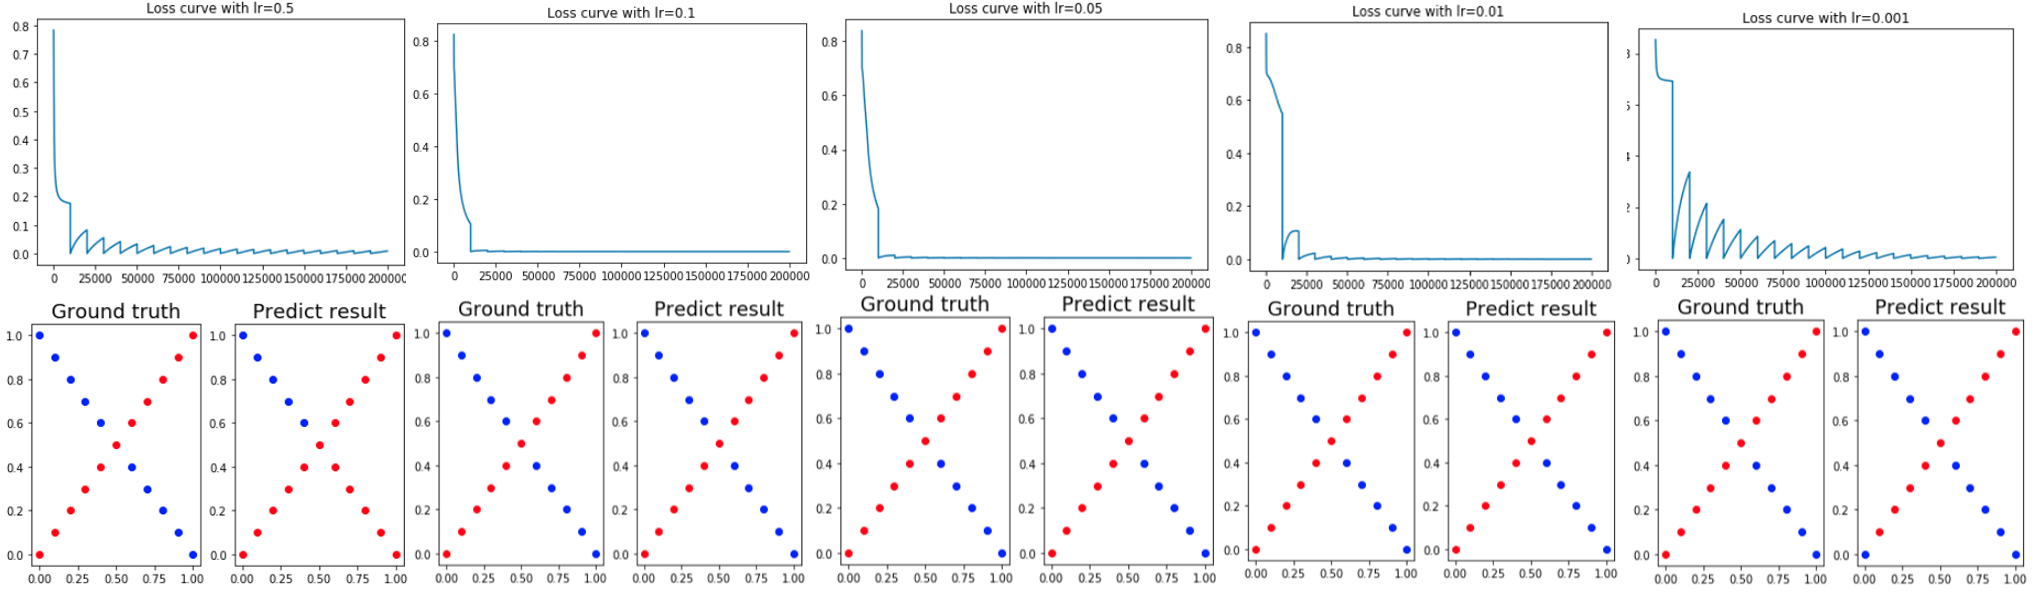
\includegraphics[scale=0.25]{lr_compare.png}
  \caption{Comparison of Learning Rate}
  \label{fig:lr_com}
\end{figure}
\begin{figure}
  \centering
  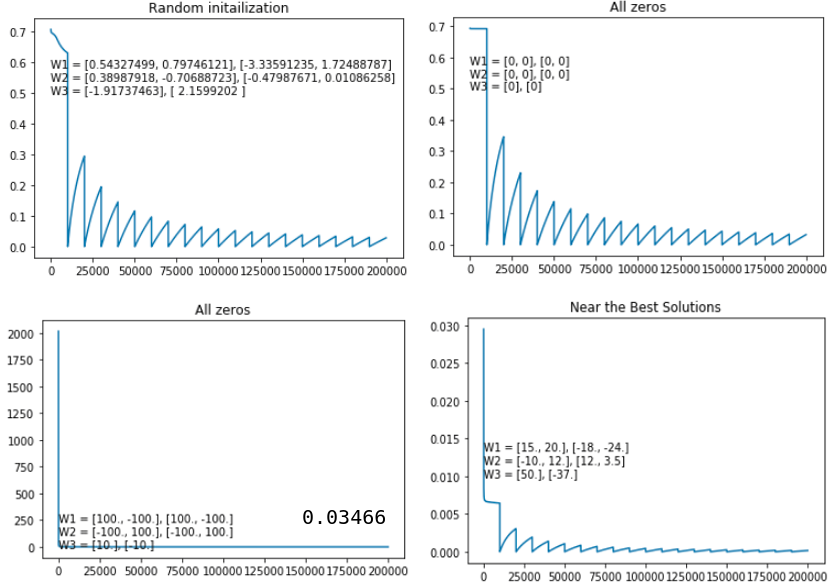
\includegraphics[scale=0.4]{initial_compare.png}
  \caption{Comparison of Different Initialization}
  \label{fig:init}
\end{figure}
\section{Discussion} \label{sec:discuss}
 
\paragraph{Matrix Expression of Gradient}
In Equation~\ref{eq: L_to_W1}, Equation~\ref{eq: L_to_W2} and Equation~\ref{eq: L_to_W3}, we show the gradients of each element to the loss function, which is complicated and hard to scale up, imaging that now we have a input layer with 100-channel input and 100-channel output, then we have to compute 10000 equations! Scalar computation not only complicated but also computation heavily compare to matrix computation. Since not familiar with matrix calculus, I met dimension error when do matrix dot product. I chose scalar computation after I couldnot find any solution.
\paragraph{Will Add Bias Term Enhance the Model?}
Since the dataset is pretty easy to train, whether or not add bias term seems not effect the power of the model. For more complex dataset, the absence of bias may affect the performance of the model. Fortunately, we can choose whether to add bias in the fully connected layer in firmware like Pytorch, make us easier to observe the differences.

\end{document}
